\documentclass[conference]{IEEEtran}
\IEEEoverridecommandlockouts

\usepackage{cite}
\usepackage{amsmath,amssymb,amsfonts}
\usepackage{graphicx}
\usepackage[caption=false,font=footnotesize]{subfig}
\usepackage{textcomp}
\usepackage{xcolor}
\usepackage{booktabs}
\usepackage{hyperref}

\setlength{\textfloatsep}{6pt}
\setlength{\floatsep}{5pt}

\begin{document}

\title{Behavioral Stability of Quantized Large Language Models Under Prompt Drift: The Resilio Evaluation Framework}

\author{
\IEEEauthorblockN{Vedant Barhate}
\IEEEauthorblockA{
\textit{School of Computing} \\
\textit{MIT ADT University} \\
Pune, India \\
vedant.barhate27@gmail.com}
\and
\IEEEauthorblockN{Yash Pandey}
\IEEEauthorblockA{
\textit{School of Computing} \\
\textit{MIT ADT University} \\
Pune, India \\
pandeyyash25@gmail.com}
\and
\IEEEauthorblockN{Achyut Yesare}
\IEEEauthorblockA{
\textit{School of Computing} \\
\textit{MIT ADT University} \\
Pune, India \\
achyutyesare886@gmail.com}
\and
\IEEEauthorblockN{Vibhor Dev}
\IEEEauthorblockA{
\textit{School of Computing} \\
\textit{MIT ADT University} \\
Pune, India \\
vibhor.101605@gmail.com}
}

\maketitle

\begin{abstract}
Large Language Models (LLMs) are actively deployed in resource-constrained environments using quantization like 8-bit and 4-bit precision, which reduces memory usage and inference costs. While these models perform well on clean benchmarks, real-world deployment frequently encounters ``Prompt Drift''-typographical errors, informal phrasing, and structural degradation.

This paper brings \textit{Resilio}, a systematic evaluation framework which investigates the interaction of model quantization and five progressive levels of prompt quality degradation. We have evaluated Llama 3.1 8B, Mistral 7B, and Phi-3 Mini using our two novel metrics: the Task Performance Score (TPS) and the Behavioral Stability Score (BSS).

These findings challenge assumptions about quantized model frailty and suggest that, for most real world applications, deployment decisions should prioritize model architecture choice and input quality control over quantization level selection.
\end{abstract}

\begin{IEEEkeywords}
Quantization, Large Language Models, Prompt Drift, Behavioral Stability, BSS, TPS, Robustness, Deployment
\end{IEEEkeywords}

\section{Introduction}

Large Language Models (LLMs) and their deployment has shifted from centralized, high-performance data centers to limited resource edge environments like mobile hardware and local workstations. This shift is driven by the need for low latency, more data privacy, and less operational costs. To make this scaling, post-training quantization (PTQ) has become the industry-standard optimization technique, which compresses model weights from 16-bit floating point (FP16) to 8-bit (INT8) or 4-bit (INT4). These methods achieve substantial memory reduction with minimal accuracy degradation on clean inputs, but they introduce a poorly understood layer of behavioral risk.

\subsection{The Phenomenon of Prompt Drift}

Standard evaluation protocols evaluate LLMs using ``ideal'' benchmarks that showcase curated, well-structured syntax. However, production environments expose models to a continuous input degradation, a phenomenon we call \textit{Prompt Drift}. Prompt Drift is the noise that occurs naturally when humans interact with AIs, with 5 levels of severity:

\begin{itemize}
\item \textbf{L1 – Typographical Noise:} Introduction of character-level errors such as misspellings, adjacency mistakes, and letter transpositions while preserving overall structure and meaning.
\item \textbf{L2 – Formatting Loss:} Removal of capitalization, punctuation, and standard formatting cues, leading to reduced structural clarity without altering core semantics.
\item \textbf{L3 – Linguistic Informality:} Incorporation of slang, abbreviations, and colloquial expressions (e.g., ``u'', ``pls'', ``bc''), introducing deviations from formal language patterns.
\item \textbf{L4 – Structural Degradation:} Breakdown of grammatical structure through word merging, spacing errors, and syntactic inconsistencies that affect sentence readability.
\item \textbf{L5 – Semantic Fragmentation:} Severe degradation characterized by incomplete phrases, truncated context, and fragmented instructions, leading to partial or ambiguous semantic representation.
\end{itemize}

\subsection{The Critical Evaluation Gap}

There still exists a gap in current AI research that is the interaction between model quantization and prompt drift remains largely unmeasured or unexplored. Standard benchmarks do not reveal how a reduction in internal numerical precision on a model's ability to parse and reason over noisy data. Quantization is a significant concern, not just in that it degrades absolute performance, but that it actively makes models more sensitive to input degradations. This amplification can lead to \textit{silent failures}, where a quantized model maintains high expressed confidence while providing factually incorrect or logically incoherent responses.

In this paper we present the \textit{Resilio} framework to address this gap. By moving beyond binary accuracy and applying multi-dimensional stability scoring, we seek to establish an empirical safety thresholds for the deployment of quantized models in noisy real-world environments.




\section{Related Work}

The deployment of Large Language Models (LLMs) on edge devices has led to a research into two previously distinct domains: computational optimization using quantization and the linguistic robustness of models under disturbances. The \textit{Resilio} framework is at the intersection of these fields.

\subsection{LLM Quantization for Efficient Deployment}

The requirement of on-device LLM execution has led to the rapid maturation of Post-Training Quantization (PTQ) methods. As stated by Dettmers \textit{et al.}~\cite{ref1}, it is observed that 8-bit matrix multiplication allows significant memory reduction with very little performance loss on curated benchmarks. Also the introduction of 4-bit quantization further extends these boundaries which enables models like Phi-3, Llama 3.1, and Mistral 7B to run within the memory constraints of mobile hardware~\cite{ref2, ref3, ref9}. 

However, previous researches has neatly studied the resource efficiency of INT4 vs. INT8 representations~\cite{ref9, ref1}, but these studies typically depends on ``clean'' input distributions. Recent work suggests that such extreme compression levels may trigger hidden instabilities or alter the model safety alignment a phenomenon sometimes termed \textit{quantization-based vulnerability}~\cite{ref9}.

\subsection{Robustness to Input Perturbations and Prompt Drift}

The sensitivity of LLMs to surface-level changes in input text is a well studied and explored challenge. Studies into typographical noise~\cite{ref11} and naturally occurring errors in training data~\cite{ref8} demonstrates that even minor character-level disturbances can produce significant variance in model output. Frameworks like PromptBench have started to standardize the measurement of model resilience against adversarial attacks~\cite{ref5}. 

Additionally, research on ``noisy instructions'' shows that the quality of the prompt is a critical determinant of zero-shot generalization~\cite{ref10}. While these insights, existing robustness studies primarily utilize full-precision (FP16 or FP32) models, resulting in a lack of understanding regarding the stability of quantized architectures under similar \textit{Prompt Drift}is  largely unmeasured~\cite{ref4}.

\subsection{Behavioral Stability and Runtime Monitoring}

As AI agents enter production, \textit{behavioral stability} has become a more critical metric than simple accuracy. This stability can be defined as the consistency of model behavior across different prompt variations~\cite{ref6}. In real-world deployment scenarios, \textit{data drift}—the variation in the distribution of user inputs over time presents a constant risk to model reliability~\cite{ref7}. 

The research community has suggested a lot of runtime monitoring strategies to detect behavioral shifts in AI systems~\cite{ref12}, there exists no unified metrics that assess stability relative to a clean baseline. The relationship between acceleration techniques and these hidden instabilities remains an open area of study~\cite{ref9}.

\subsection{Identification of Research Gaps}

A systematic review of the literature reveals a critical tripartite gap:

\begin{itemize}
\item \textbf{Isolation of Factors:} Quantization is typically evaluated on clean inputs, while robustness is tested on full-precision models. The interaction between bit-precision and input drift is largely unexplored.

\item \textbf{Absence of Graduated Drift Frameworks:} Most studies depends on binary noise conditions (clean vs.\ noisy) rather than a structured, multi-level taxonomy (L1--L5) as proposed in this work.

\item \textbf{Metric Limitations:} Standard accuracy metrics fails to capture \textit{silent failures}, where a model maintains high confidence despite producing logically inconsistent or incorrect outputs.
\end{itemize}

With the introduction of the \textit{Task Performance Score (TPS)} and \textit{Behavioral Stability Score (BSS)}, the \textit{Resilio} framework gives a multi-factor analysis of task-specific stability patterns under quantized prompt drift.






\section{The Resilio Methodology}

The working of the \textit{Resilio} framework focuses on a modular, reproducible pipeline that overcomes the gap between synthetic benchmarks and the stochastic nature of production-level input noise. There are three main steps in the methodology: creating a custom dataset, simulating object-oriented drift, and validating semantics.

\subsection{Dataset Architecture}

We use a special crafted dataset of 40 base prompts to make it easier to do a detailed analysis and study of model stability. These prompts are grouped in a way that makes them look like common language problems, but they were made specifically to test certain behavioral abilities in Large Language Models:

\begin{itemize}
\item \textbf{Reasoning:} 10 prompts engineered to evaluate multi-step mathematical logic and sequential deduction.
\item \textbf{Logical Inference:} 10 prompts structured to assess complex deductive reasoning and syllogistic consistency.
\item \textbf{Question Answering:} 10 prompts focused on the precision of factual retrieval and context-window utilization.
\item \textbf{Sentiment Classification:} 10 prompts designed to measure the robustness of pattern recognition under lexical noise.
\end{itemize}

\subsection{OOP-based Drift Generation Framework}

In the \textit{Resilio} framework, the drift generation engine is implemented as an object-oriented module, enabling modular and extensible application of transformations. To ensure statistical diversity, each base prompt was instantiated across 16 distinct variants per degradation level.

The framework shows \textit{Prompt Drift} into a five level of degradations:

\begin{itemize}
\item \textbf{L1 (Character-level Perturbation):} Simulates typographical errors via keyboard adjacency mapping and character transpositions.
\item \textbf{L2 (Form Degradation):} Implements systematic removal of casing, standard punctuation, and formal whitespace.
\item \textbf{L3 (Linguistic Shift):} Replaces formal lexical units with slang, non-standard abbreviations, and colloquial expressions.
\item \textbf{L4 (Grammatical Breakdown):} Induces word merging, omission of essential function words, and overall syntactic collapse.
\item \textbf{L5 (Structural Truncation):} Combines aggressive informality with content reduction, forcing the model to infer intent from fragmented inputs.
\end{itemize}

\subsection{Mathematical Validation of Realism}

To make sure that the drifts generated represent realistic ``noisy'' input rather than incoherent gibberish, we mathematically validate the quality of perturbations using the \texttt{all-MiniLM-L6-v2} SentenceTransformer model. We calculate the cosine similarity between the clean baseline (L0) and each drifted variant.

Formally, for embedding vectors $\mathbf{u}$ (clean prompt) and $\mathbf{v}$ (drifted prompt), cosine similarity is defined as:

\begin{equation}
\text{CosineSimilarity}(\mathbf{u}, \mathbf{v}) =
\frac{\mathbf{u} \cdot \mathbf{v}}{\|\mathbf{u}\| \, \|\mathbf{v}\|}
\end{equation}

The generated variants are required to be in below given ranges:

\begin{itemize}
\item \textbf{L1:} 93.2\% similarity (high surface-level accuracy)
\item \textbf{L2:} 88.1\% similarity (loss of structural cues)
\item \textbf{L3:} 83.4\% similarity (lexical divergence)
\item \textbf{L4:} 77.8\% similarity (syntactic fragmentation)
\item \textbf{L5:} 71.5\% similarity (boundary of semantic coherence)
\end{itemize}

This ensures that the \textit{Resilio} framework provides a properly controlled and semantically grounded stress test for evaluating quantized LLMs robustness.





\section{Metric Formulation (TPS \& BSS)}

The primary analytical innovation of the \textit{Resilio} framework is its shift from binary accuracy measures to a multi-dimensional reliability analysis. Through the separation of peak performance from structural integrity, we propose a two-metric approach that reflects the nuanced breakdown of quantized models.

\subsection{Task Performance Score (TPS): The 5-Factor Behavioral Matrix}

Conventional benchmarking struggles to detect "silent failures" - cases where a model retains linguistic coherence while suffering logical or factual degradation. To measure these phenomena, we score each response along a weighted five-dimensional behavioral matrix:

\begin{itemize}
\item \textbf{Factual Correctness (FC):} Comparing the model's final answer against metadata.
\item \textbf{Logical Correctness (LC):} Confirmation of deductive validity and mathematical correctness of intermediate steps.
\item \textbf{Reasoning Coherence (RC):} Verification of structural soundness and temporal clarity of the explanation.
\item \textbf{Sentiment Correctness (SC):} Verification of label correctness for pattern matching and classification problems.
\item \textbf{Manner of Language (ML):} A calibration score that assesses if language confidence is consistent with the accuracy of the output.
\end{itemize}

The Task Performance Score (TPS) is computed as:

\begin{equation}
TPS = \sum_{i=1}^{5} \left( w_i \cdot \text{Score}_i \right)
\end{equation}

where $w_i$ denotes task-specific weight coefficients. These weights are dynamically adjusted; for example, Logical Correctness ($LC$) is prioritized in reasoning tasks, while Sentiment Correctness ($SC$) is emphasized in classification settings.

\subsection{Behavioral Stability Score (BSS)}

TPS reflects absolute performance, but the \textit{Behavioral Stability Score (BSS)} reflects stability to input degradation. By normalizing degraded performance against a clean baseline, BSS provides a relative stability index independent of model scale.

For a given drift level $d$, BSS is defined as:

\begin{equation}
BSS_d = \frac{\overline{TPS}_d}{TPS_0}
\end{equation}

where $\overline{TPS}_d$ represents the mean Task Performance Score across all variants at drift level $d$, and $TPS_0$ denotes performance on the clean baseline (L0).

\subsection{Stability Threshold and Behavioral Collapse}

One key empirical contribution of this study is the discovery of a stability threshold at $BSS < 0.7$. This threshold separates ``safe degradation'' from \textit{behavioral collapse}.

The 0.7 threshold is justified by the observed gap between language fluency and factual correctness. Below this threshold, the incidence of ``silent failures'' rises dramatically: models score highly on Manner of Language ($ML$), but show substantial degradation in Factual Correctness ($FC$) and Logical Correctness ($LC$).

The establishment of this threshold by the \textit{Resilio} framework offers a safety measure for setting quantization levels in practical deployment settings.





\section{Experimental Setup and Implementation}

The empirical research of the \textit{Resilio} framework was done on a large-scale compute infrastructure that tested the interactive relationships between model design, quantization, and input disturbance. The implementation of setup was designed to maintain a level playing field for all tests to ensure that quantization and drift were the only variable factors at play.

\subsection{Technical Infrastructure and Model Configurations}

This study used a high-performance compute environment with the use of \textit{Hugging Face} ecosystem and the \textit{BitsAndBytes} library for precision management. We selected three open-source models which represents diverse parameter scales and architectural designs: \textit{Llama 3.1 8B}, \textit{Mistral 7B}, and \textit{Phi-3 Mini}. Each model was setted up across three distinct quantizations:

\begin{itemize}
\item \textbf{FP16:} The 16-bit floating-point baseline.
\item \textbf{INT8:} 8-bit quantization using vector-wise quantization logic.
\item \textbf{INT4:} 4-bit quantization with double quantization enabled for maximum memory efficiency.
\end{itemize}

To maintain internal validity, we enforced consistent generation parameters across all 5,760 total inferences, utilizing a temperature of 0.7, a top-$p$ value of 0.9, and a maximum token limit of 350.

\subsection{The LLM-as-Judge Evaluation Pipeline}

Manual annotation of 5,760 multi-factor responses was determined to be logistically unfeasible; we therefore engineered an automated evaluation pipeline utilizing \textit{GPT-OSS 20B} as a neural rater, accessed via the \textit{Groq API}. This \textit{LLM-as-Judge} system was prompted with a structured JSON protocol to extract a five-dimensional scoring vector—Factual Correctness (FC), Logical Correctness (LC), Reasoning Coherence (RC), Sentiment Correctness (SC), and Manner of Language (ML)—for each response.

To resolve technical bottlenecks and ensure data integrity, the pipeline implemented:

\begin{itemize}\item \textbf{Asynchronous Threading:} Designed to maintain an optimal throughput of 30 requests per minute (RPM) and manage API rate limits during inference.
\item \textbf{Contextual Grounding:} Each evaluation request included the original clean prompt and ground-truth metadata to prevent evaluator hallucination.
\item \textbf{Memory Management:} Automated GPU offloading and memory cleaning were utilized between quantization cycles to prevent VRAM fragmentation during local INT4/INT8 testing.
\end{itemize}

\subsection{TPS and BSS Computation \& Visualization}

After the evaluation stage, the scoring vectors were used to calculate the main metrics: Task Performance Score (TPS) and Behavioral Stability Score (BSS). The TPS for each individual response was obtained as a weighted sum of the five evaluation factors, with category-specific weights to account for the different types of Reasoning, Logic, Question Answering and Classification tasks.

The Behavioral Stability Score (BSS) was then calculated at each level of drift as the quotient between the average TPS of the prompt degradation variants ($\overline{TPS}_d$) and the TPS of the clean baseline ($TPS_0$). This allowed us for comparing the degradation trends relative to performance, regardless of model with quantization.

To facilitate this analysis, the results were structured across dimensions of model architecture, quantization level, task category, and drift levels. For visualizations use of graphs such as line plots to trace BSS trajectories, bar charts to assess prompt-level variability, and heatmaps to detect category-specific stability patterns, were used to look at degradation patterns and the effects of quantization.


This multi-level approach allowed for proper interpretation of behavioral stability of LLMs under all experimental conditions.






\section{Results, Analysis, and Discussion}

% --- FIGURE 1: FULL WIDTH (INTRO CONTEXT) ---
\begin{figure*}[t]
\centering
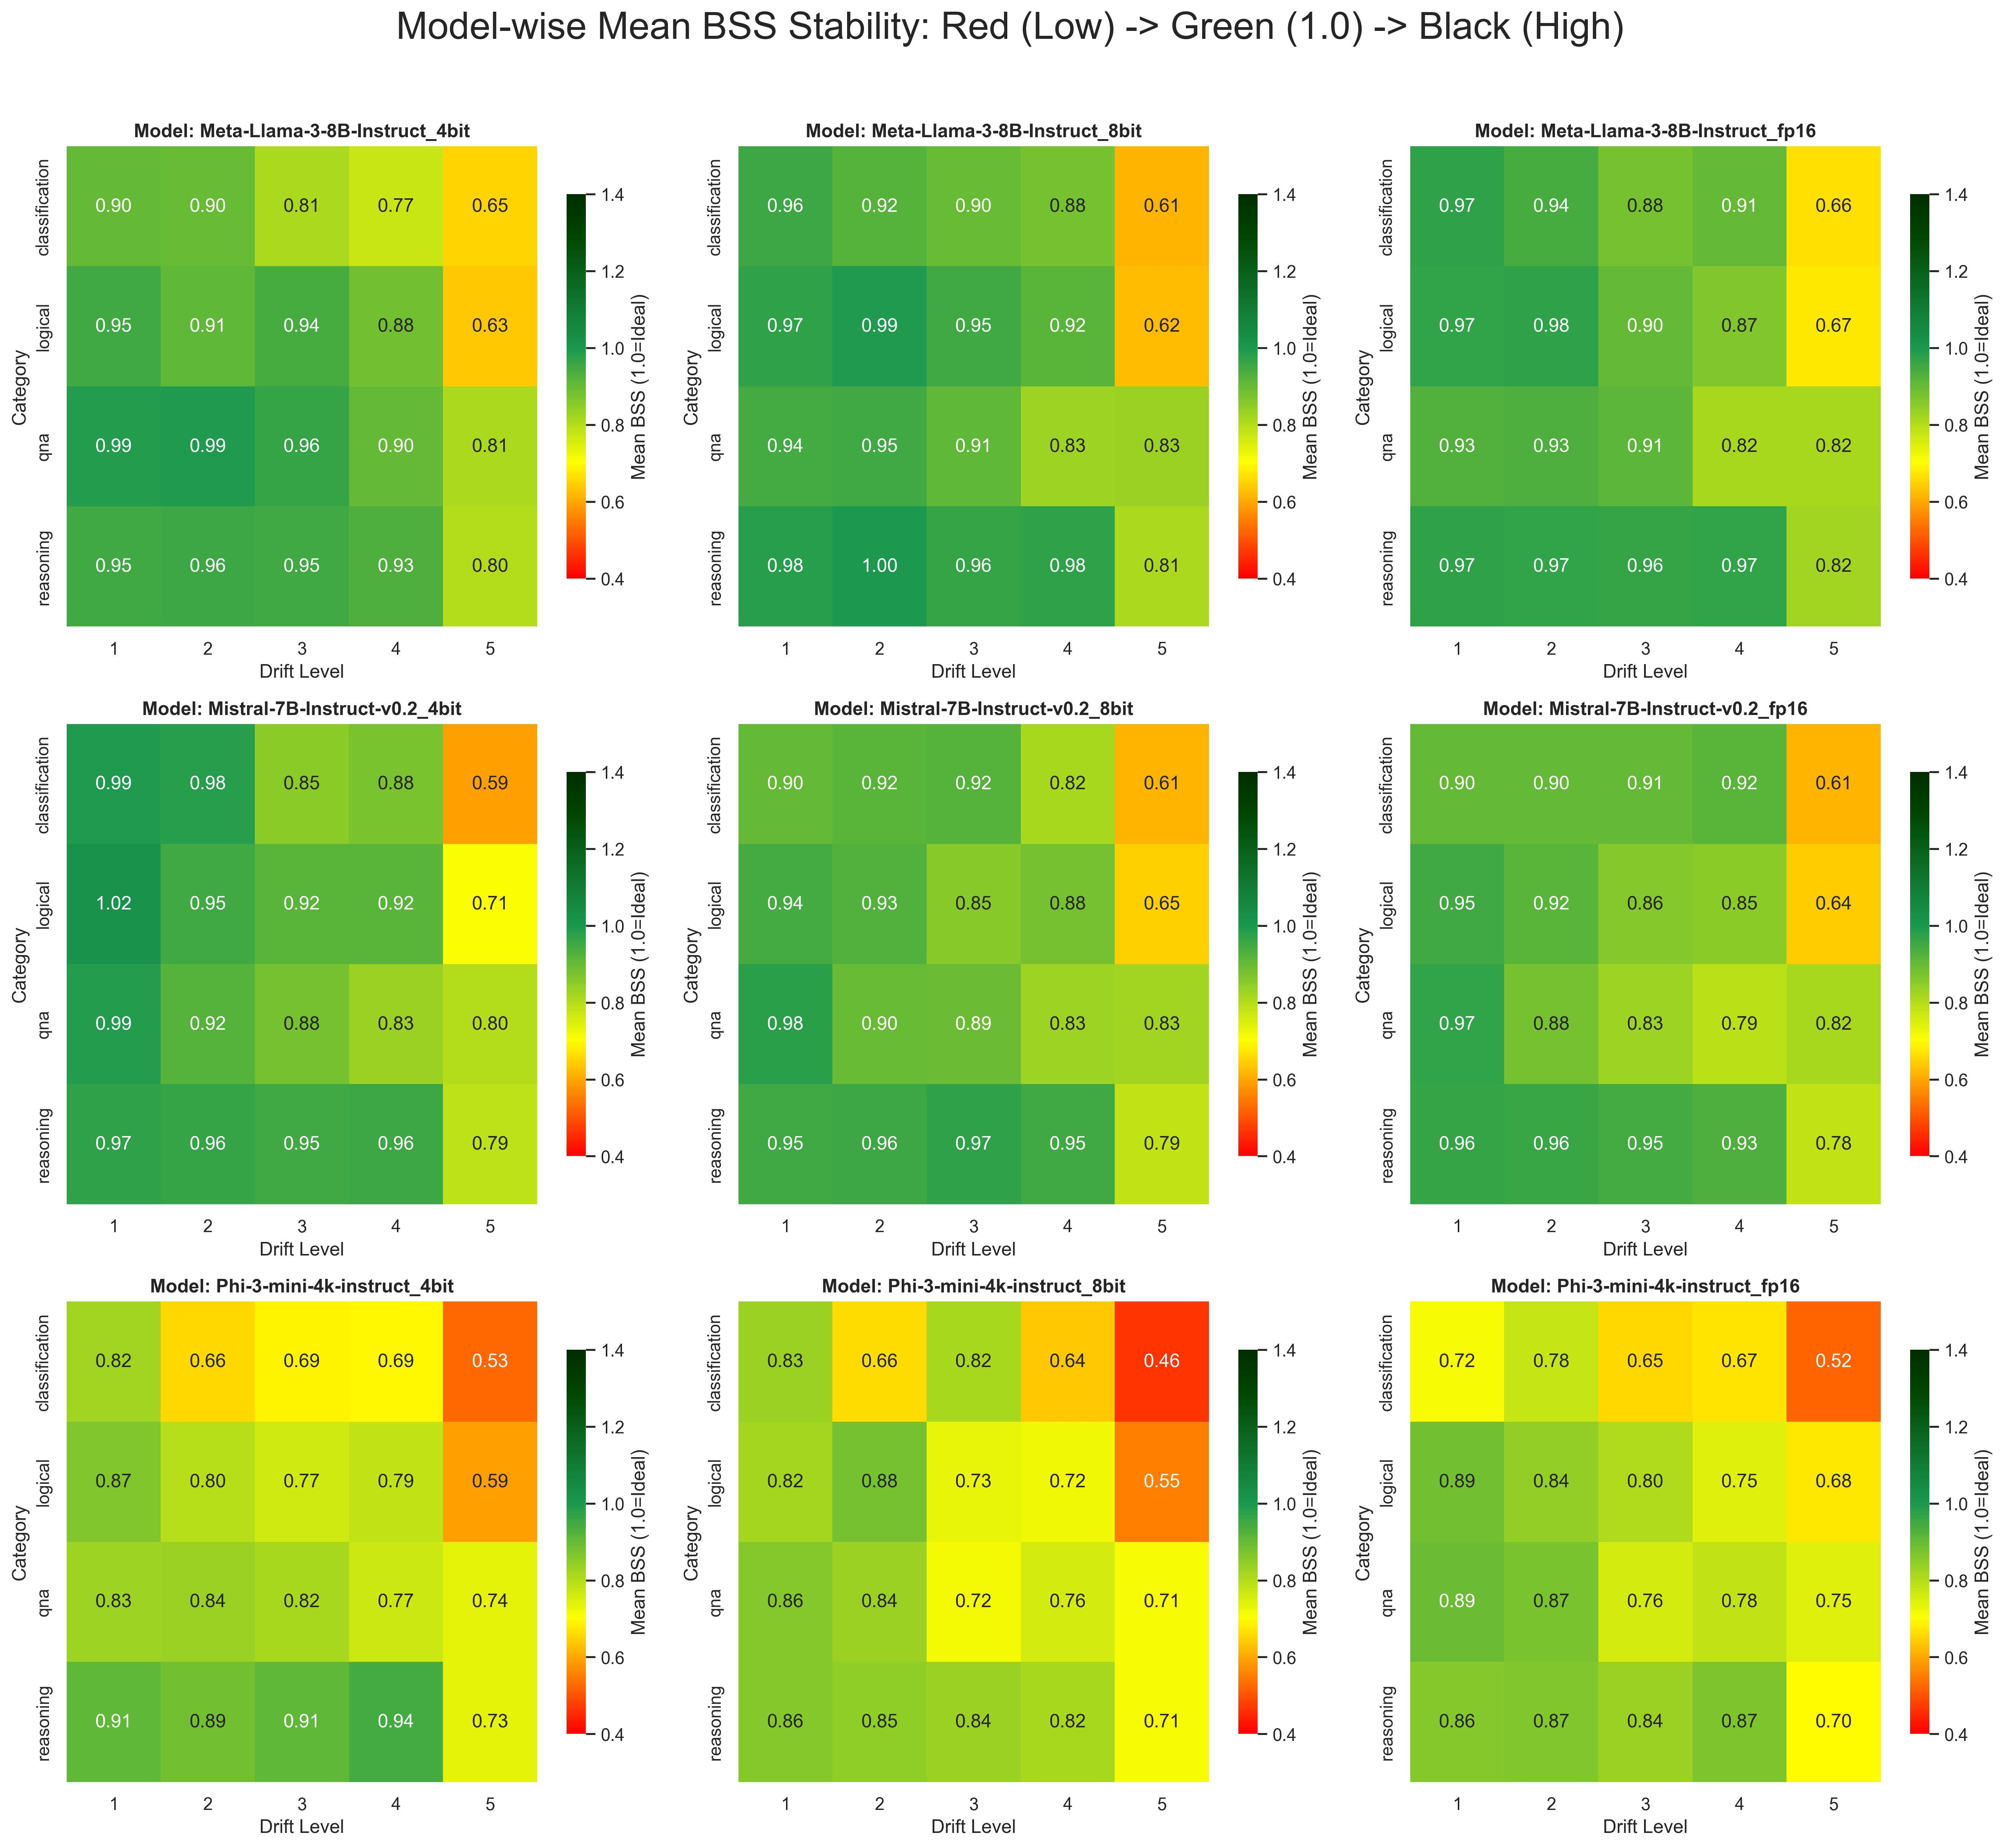
\includegraphics[width=0.85\textwidth]{modelwise_mean_bss.png}
\caption{All models exhibit progressive degradation with increasing drift severity. INT4 configurations demonstrate an earlier onset and steeper decline trajectory, particularly in reasoning tasks.}
\label{fig:modelwise_bss}
\end{figure*}

As shown in Fig.~\ref{fig:modelwise_bss}, all models exhibit a gradual degradation in stability as drift increases, with INT4 configurations collapsing significantly earlier.

% --- FIGURE 2 + 3 (SIDE-BY-SIDE) ---
% --- FIGURE 2 + 3 (SIDE-BY-SIDE) ---
\begin{figure*}[t]
\centering
\subfloat[Category-wise BSS]{
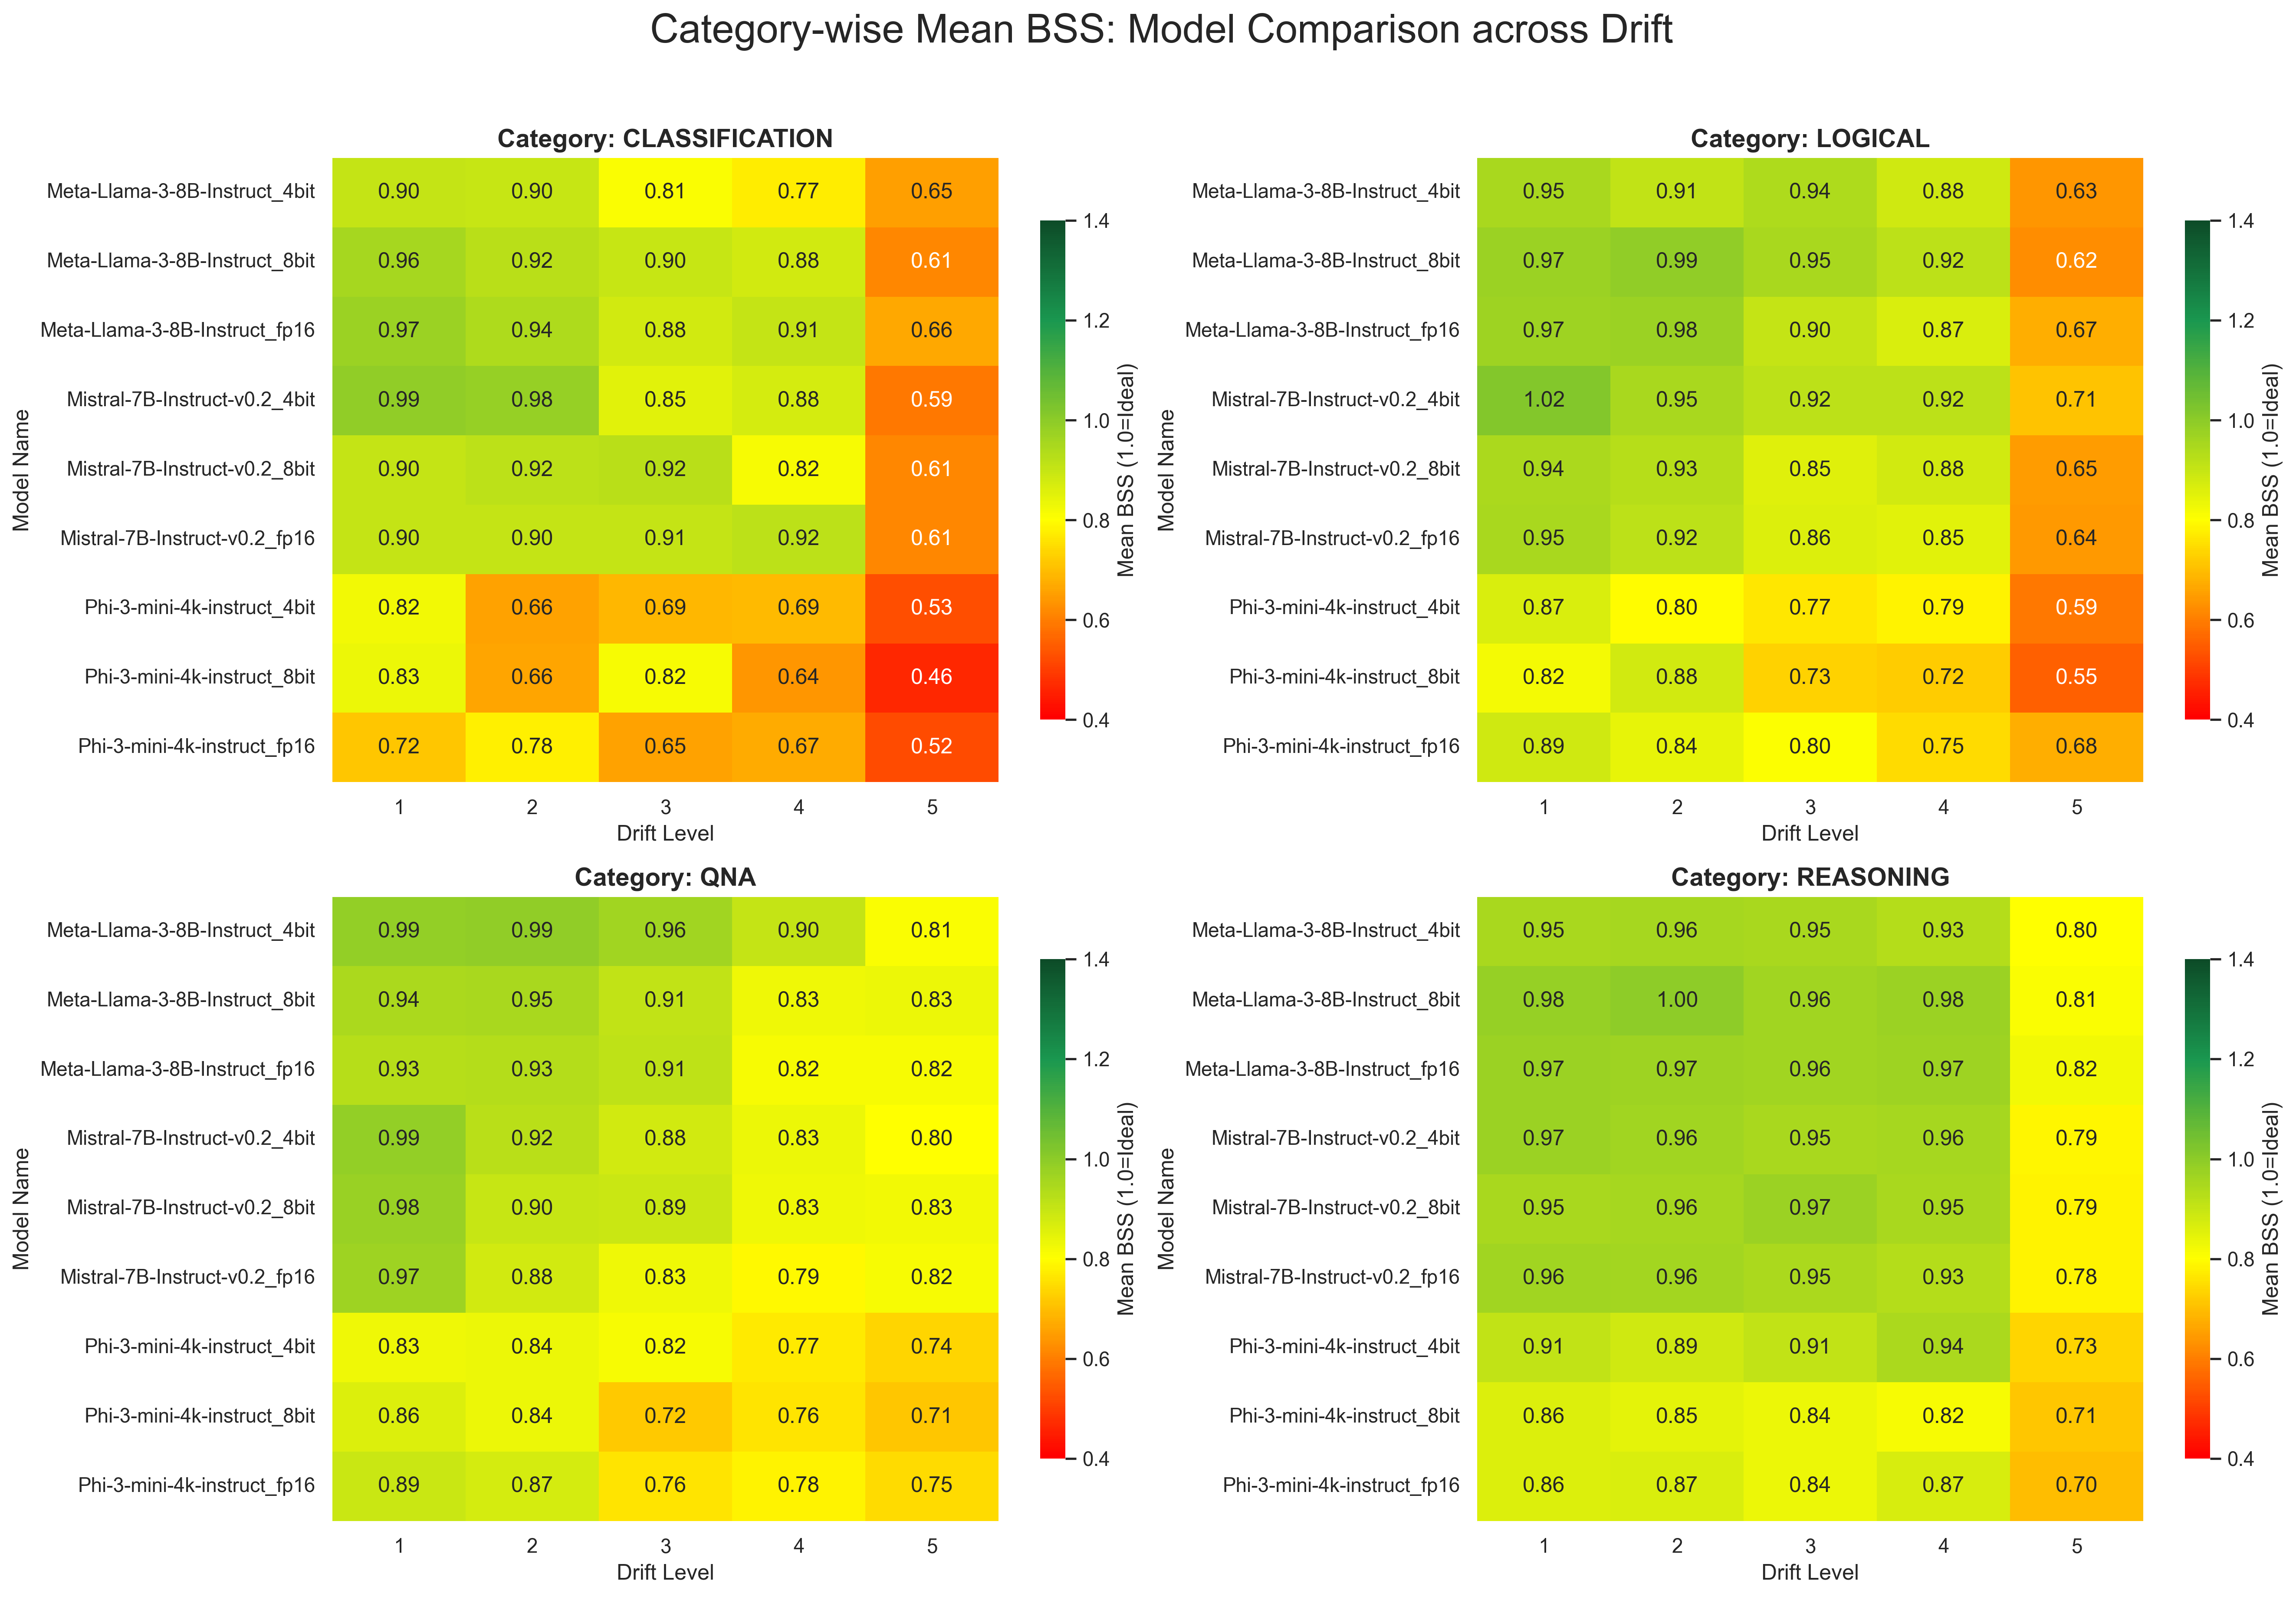
\includegraphics[width=0.45\textwidth]{categorywise_mean_bss.png}
\label{fig:category_bss}
}
\hfill
\subfloat[Aggregated Quantization Impact]{
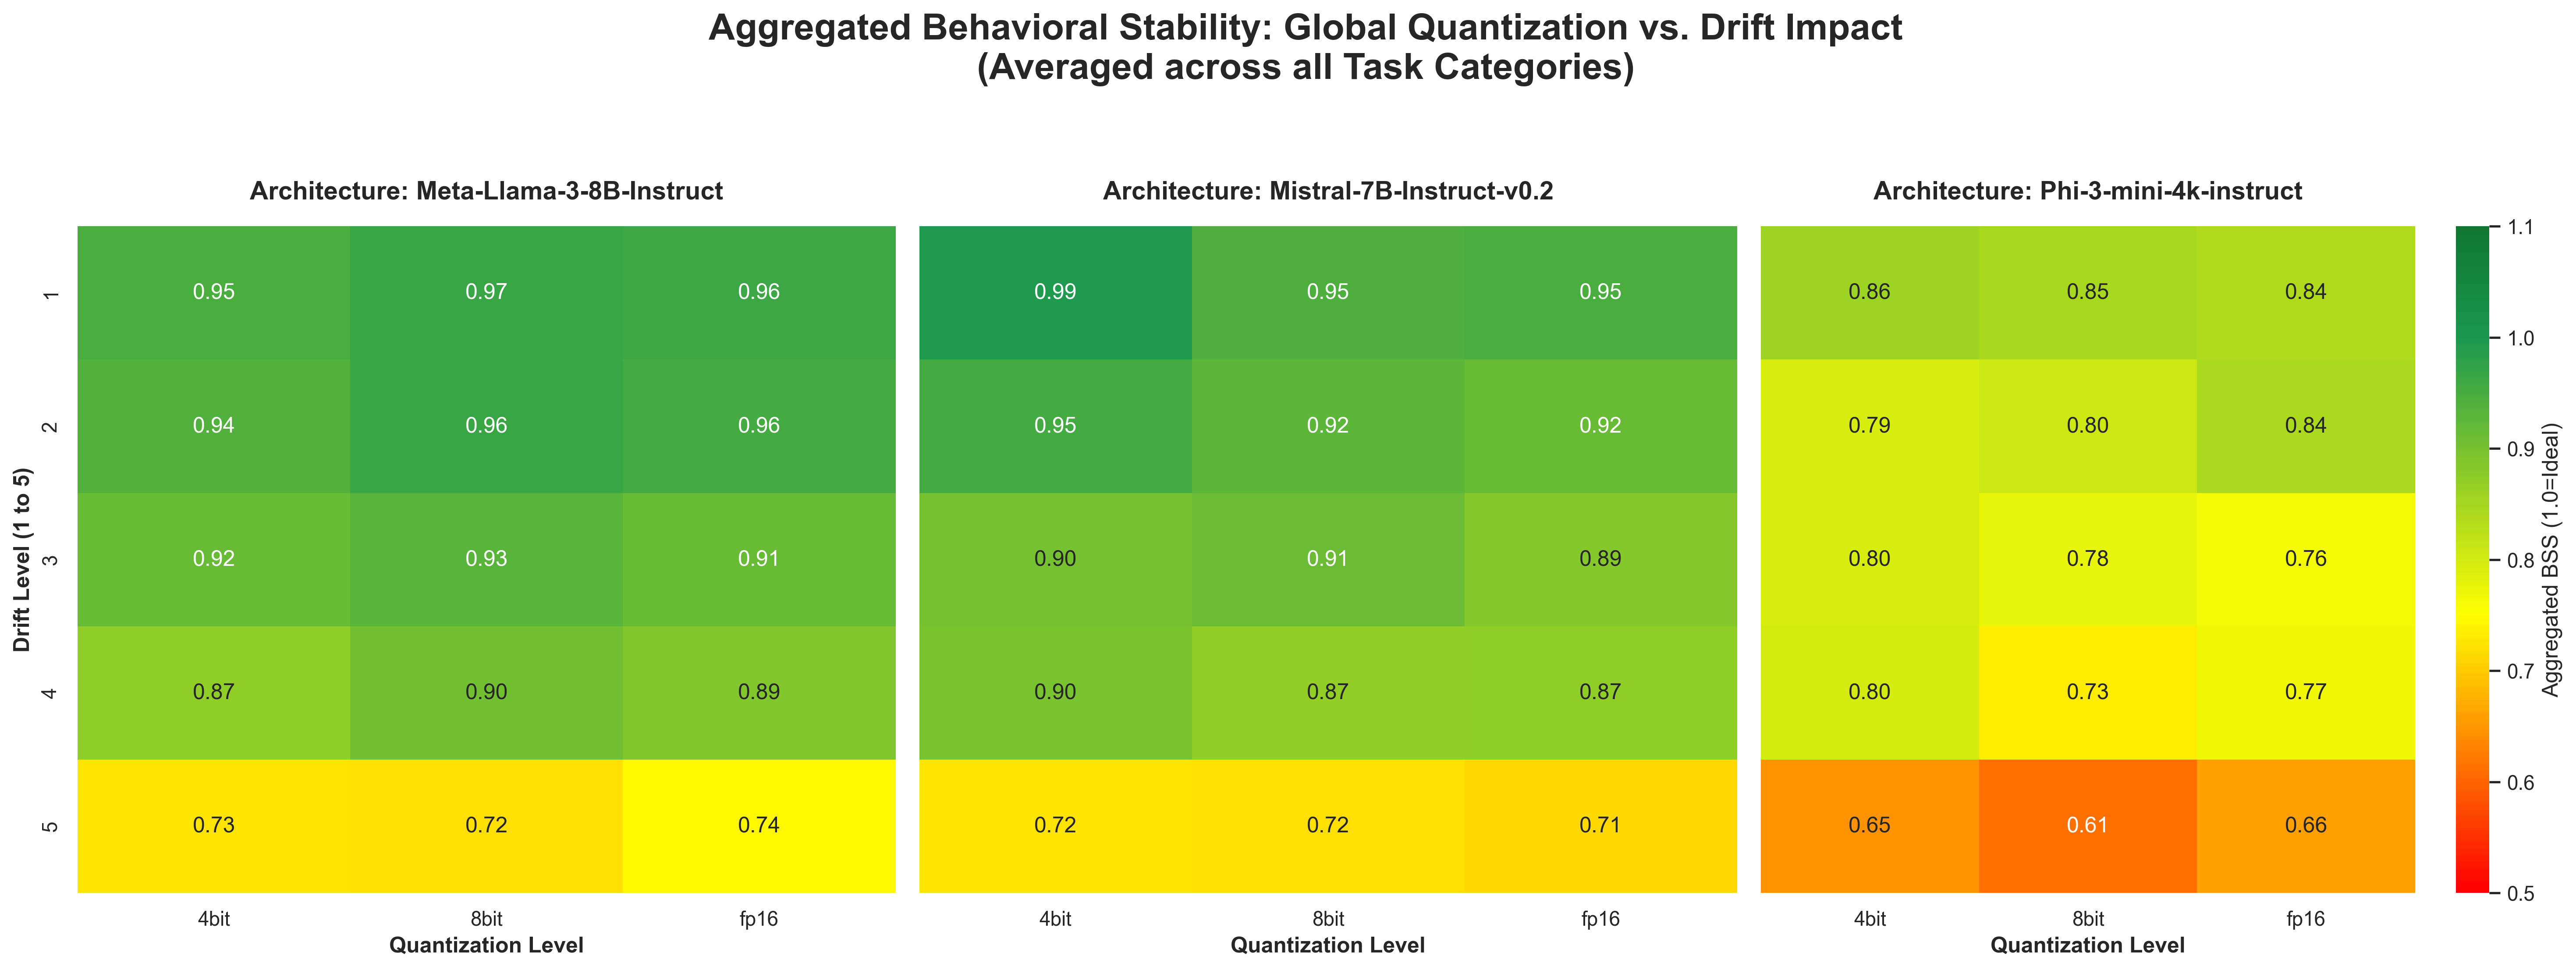
\includegraphics[width=0.45\textwidth]{aggregated_quantization_bss.png}
\label{fig:agg_quant_bss}
}
\caption{(a) Category-wise BSS showing task-dependent robustness differences. (b) Aggregated quantization trends demonstrating a consistent decline in stability with reduced precision.}
\end{figure*}

Fig.~\ref{fig:category_bss} highlights task-specific divergence across categories, while Fig.~\ref{fig:agg_quant_bss} shows the global degradation trend across quantization levels.

% --- FIGURE 4 + 5 (SIDE-BY-SIDE) ---
\begin{figure*}[t]
\centering
\subfloat[Quantization Gap]{
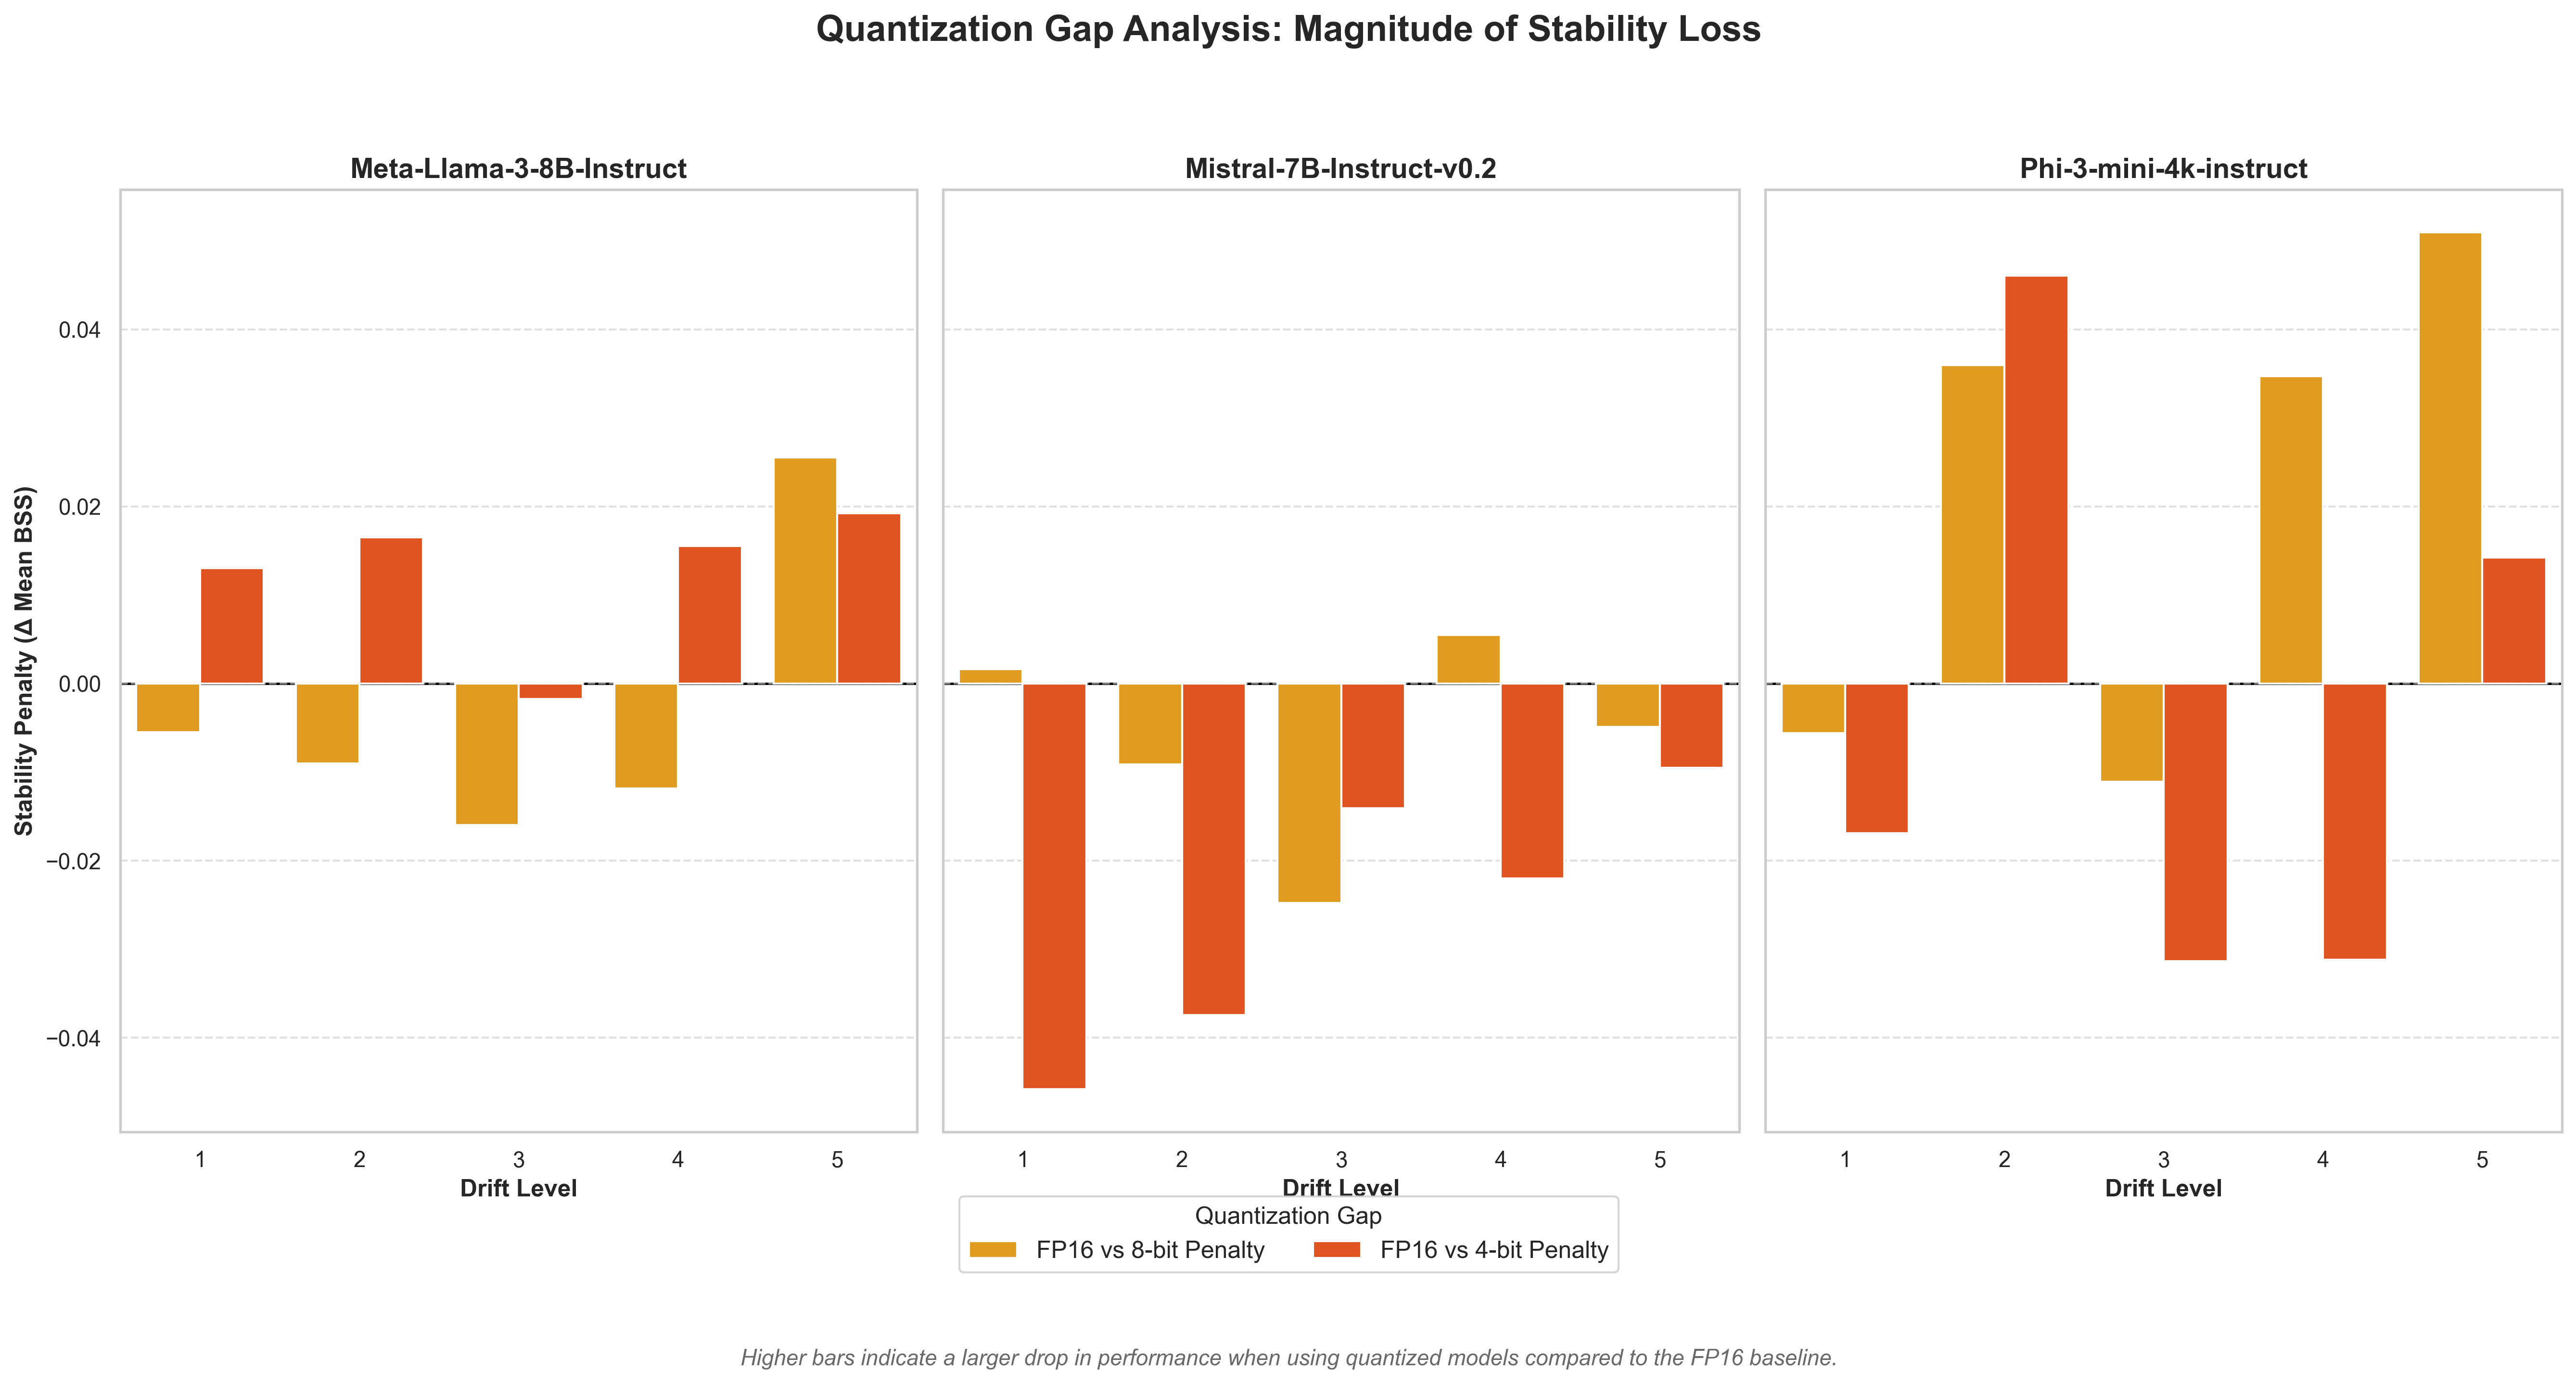
\includegraphics[width=0.45\textwidth]{quantization_gap_analysis.png}
\label{fig:quant_gap}
}
\hfill
\subfloat[Statistical Significance]{
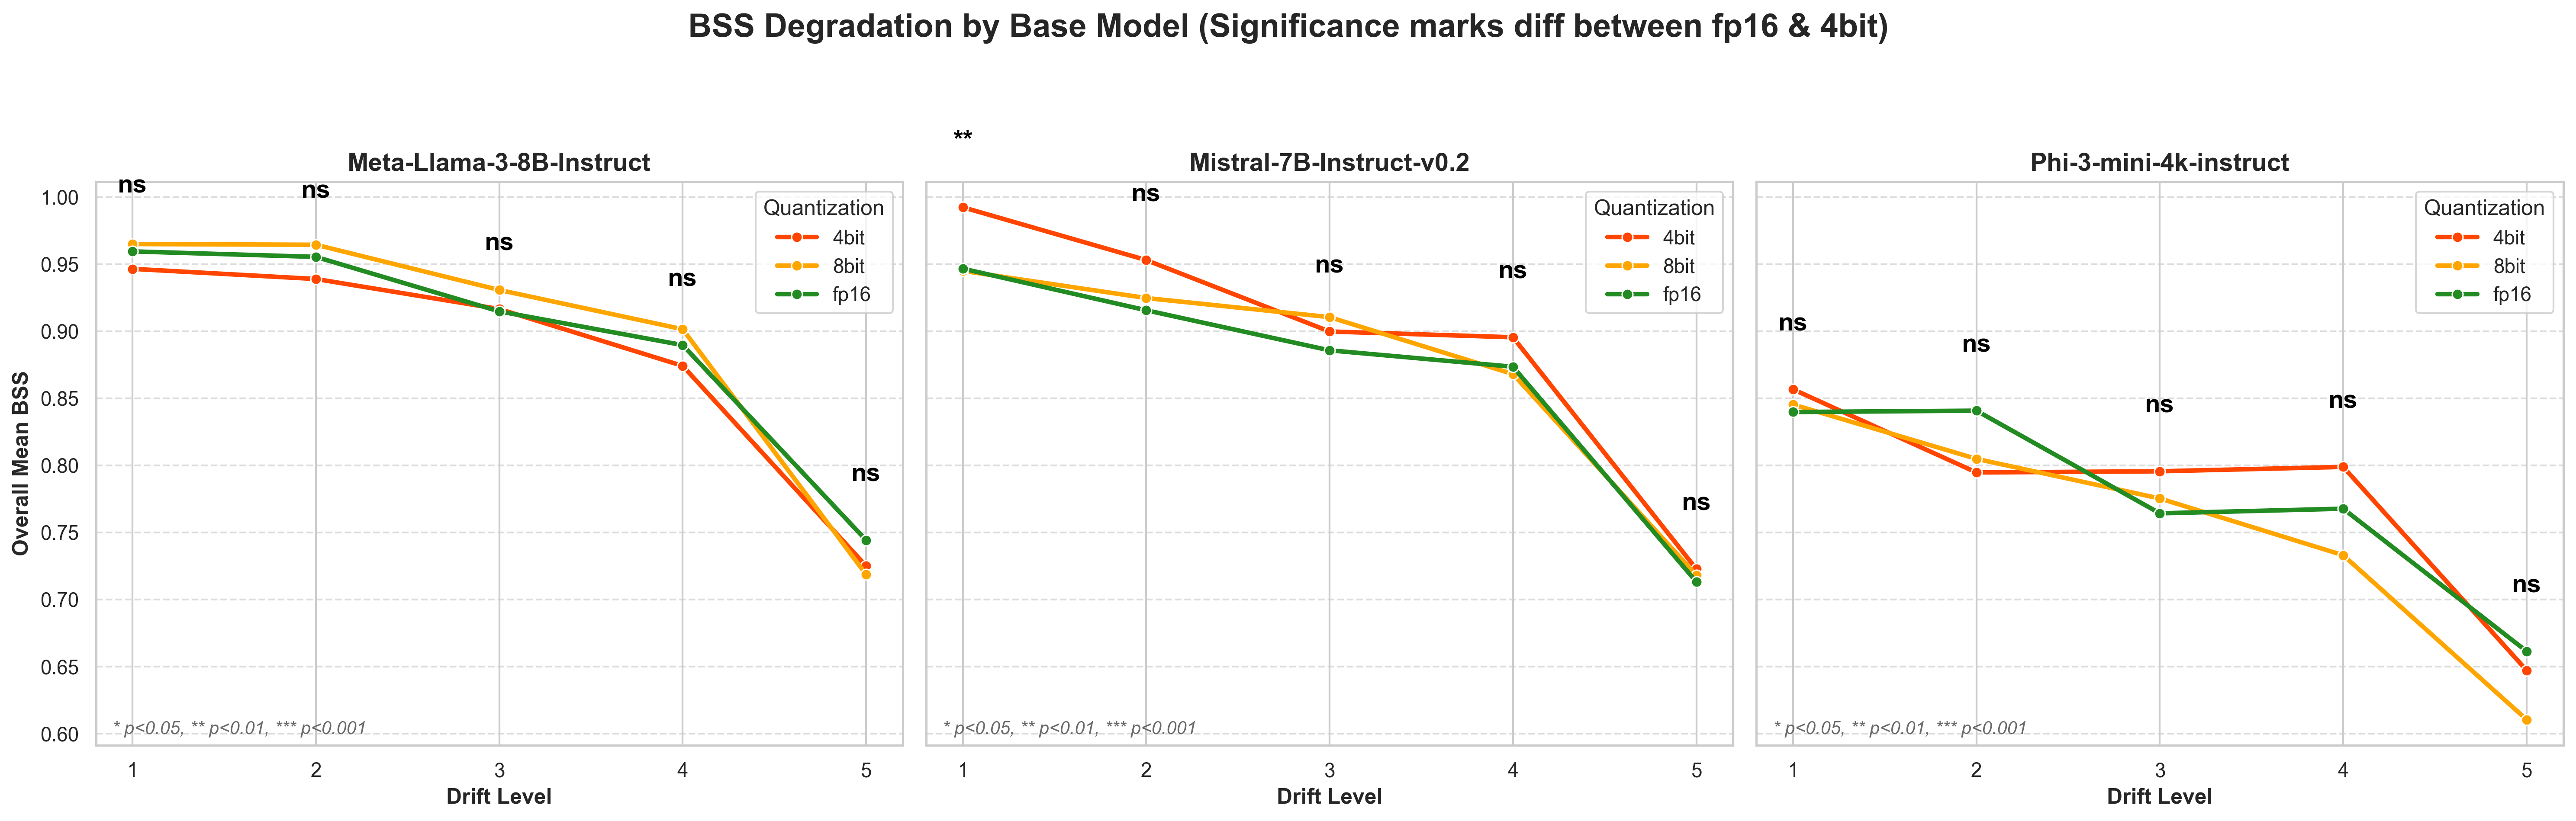
\includegraphics[width=0.45\textwidth]{bss_with_significance.png}
\label{fig:bss_significance}
}
\caption{(a) Quantization gap analysis highlighting disproportionate stability loss in INT4 models. (b) Statistical validation confirming that degradation trends are significant across drift levels.}
\end{figure*}

Fig.~\ref{fig:quant_gap} demonstrates that INT4 degradation is disproportionately higher, while Fig.~\ref{fig:bss_significance} confirms statistical reliability.

% --- FIGURE 6: FINAL INSIGHT (FULL WIDTH) ---
\begin{figure*}[t]
\centering
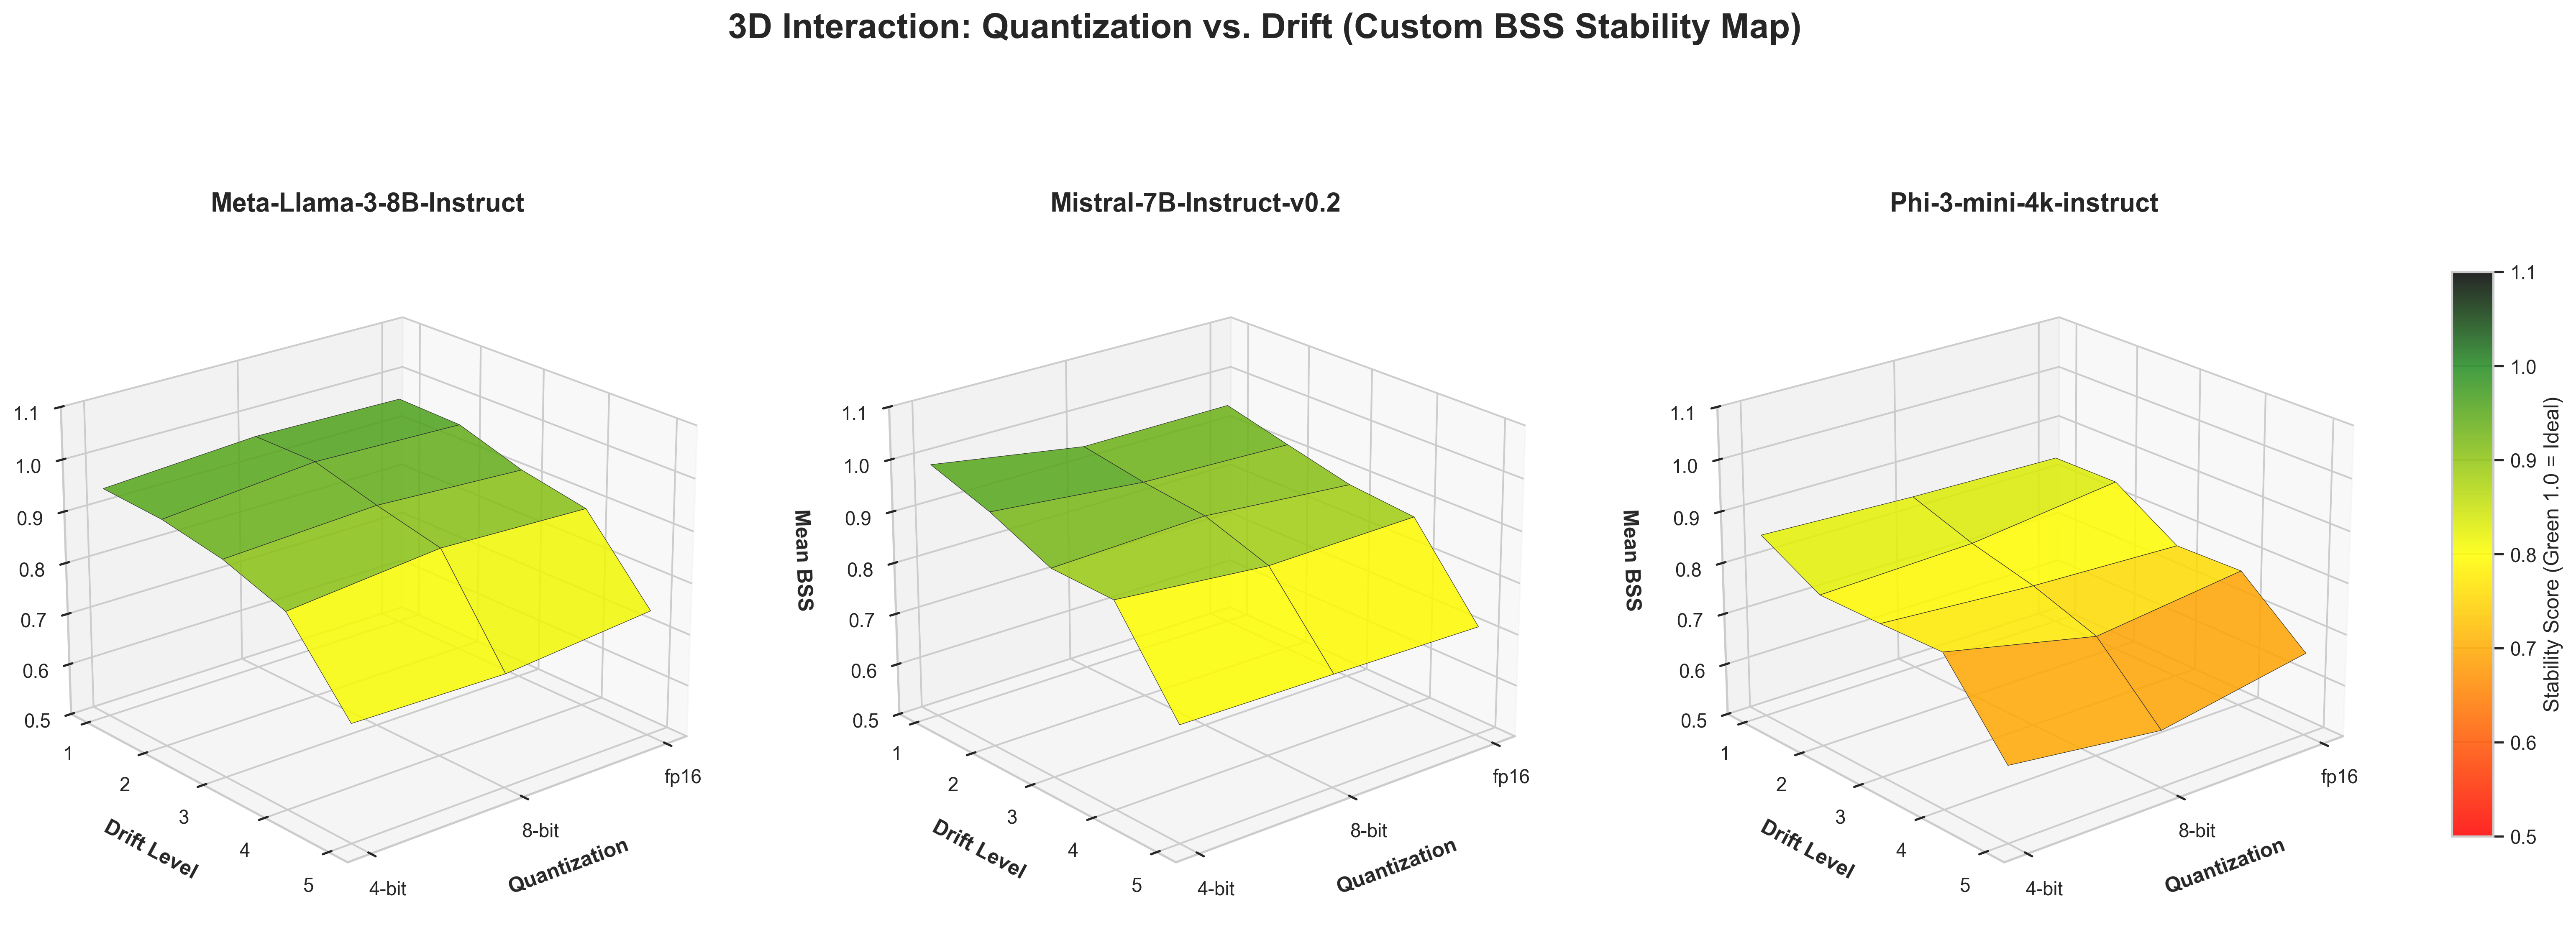
\includegraphics[width=0.85\textwidth]{bss_3d_interaction.png}
\caption{3D interaction between model architecture, quantization level, and drift severity, illustrating the compounded impact of compression and input degradation on behavioral stability.}
\label{fig:bss_3d}
\end{figure*}

Fig.~\ref{fig:bss_3d} illustrates the higher-order interaction between architecture, quantization, and prompt drift.

Our empirical study which consisted of 5,760 model response configurations shows a complex and non-linear interaction between numerical and linguistic behavioral stability. Our main focus is on three key observations: the Quantization Amplification effect, task-specific Fragility, and the rise of \textit{silent failures} in quantized models.

\subsection{The Quantization Amplification Effect}

One of the findings of this research is that the \textit{Quantization Amplification} effect, where low bit-precision does not only lower absolute performance but also actively speeds up the rate of behavioral degradation under input noises.

Our findings show a consistent but subtle Quantization Amplification effect. The absolute gap in BSS between INT4 and FP16 configurations is small (1-3 percentage points) at lower drift levels, but more significant at higher drift levels (L4-L5) for reasoning-heavy tasks. In Phi-3 Mini, the rate of degradation at INT4 is more rapid than FP16 and reaches BSS $< 0.75$ at L5, whereas FP16 has BSS $> 0.80$ in classification tasks. This non-linear increase in the slope of degradation (as opposed to a substantial absolute difference) forms the basis of our amplification effect.

This suggests that at 4-bit the model shows a lower tolerance for noise in its responses. The impact is not a sudden failure of the model rather it is accelerated degradation and more rapid degradation rate under high drift levels, especially for models with fewer parameters architecture such as Phi-3 Mini.

\subsection{Task-Specific Fragility: Reasoning vs. Classification}

Our findings show that BSS is highly task-specific, as it can be observed from category-specific BSS trends. There is a clear separation between pattern matching and computational reasoning tasks:

\begin{itemize}
\item \textbf{Logical and Reasoning Fragility:} Tasks needing multi-step inference (e.g., GSM8K and LogiQA) are the most fragile tasks. These tasks reach their \textit{behavioural collapse threshold} ($BSS < 0.7$) at L3 drift with INT4. The imprecision affects the consistency of chain-of-thought reasoning, in which a single token shift can alter the reasoning path.
\item \textbf{Resilience of Classification:} By contrast, sentiment classification (SST-2) is very robust. Even with INT4 models, the $BSS > 0.8$ with L3 drift for most models. This implies classification is based on global semantic features, which are not as affected by local changes caused by quantization.
\end{itemize}

\subsection{The Silent Failure Phenomenon and Calibration Loss}

A potential safety issue was discovered in this study which highlights the existence of \textit{silent failures}, which refers to a lack of proper relationship between language fluency and accuracy.

Our multi-factor scoring reveals that while \textit{Manner of Language (ML)} scores are high, \textit{Factual Correctness (FC)} and \textit{Logical Correctness (LC)} decrease effectively in high drift levels. Like in INT4 quantization setups, models often produce linguistically fluent and confident answers that are factually incorrect and/or logically inconsistent.

This \textit{confidence-accuracy mismatch} is an important deployment topic to discuss upon. It is possible to manage failure with low confidence, but failure with high confidence possess a significant risk in real-world deployment scenarios.

\subsection{Discussion: Implications for Deployment}

Our results findings shows the existence of a practical \textit{stability ceiling} for stability of quantized models. While INT4 quantization remains feasible for low-complexity classification tasks under moderate noise, it is simply unsuitable for reasoning-intensive tasks without proper input preprocessing.

These results demonstrate a key design trade-off in this models and that is the benefits of memory and efficiency through aggressive quantization come at the cost of a higher risk of model collapsing under real-world input prompting scenarios. Thus, the users need to weigh the gains from compression against the need for robustness when using LLMs in production environments.





\section{Deployment Guidelines}

The findings from the \textit{Resilio} study provides a solid evidence base for optimizing the trade-off between computational efficiency and behavioral stability. We offer a deployment decision matrix to help practitioners make informed decisions..

\subsection{Deployment Decision Matrix}

Based on the observed stability thresholds ($BSS < 0.7$), we recommend the following precision-task mapping for production environments:

\begin{table}[t]
\centering
\caption{Deployment Decision Matrix}
\begin{tabular}{|p{2.2cm}|p{2.2cm}|p{3.5cm}|}
\hline
\textbf{Task Category} & \textbf{Precision} & \textbf{Operational Constraint} \\
\hline
Reasoning / Logic & FP16 / INT8 & INT4 viable only if input similarity $> 90\%$ \\
\hline
Fact-Retrieval (QA) & INT8 & Safe for moderate drift; INT4 requires normalization \\
\hline
Classification & INT4 & Robust under high drift conditions \\
\hline
Safety-Critical & FP16 & Avoid quantization to prevent silent failures \\
\hline
\end{tabular}
\end{table}

\subsection{Strategic Recommendations for Practitioners}

\begin{enumerate}
\item \textbf{Prioritize Input Normalization:} For reasoning-intensive tasks, applying a lightweight spell-correction or grammar-normalization layer prior to inference can significantly improve stability in low-precision models.
\item \textbf{Monitor Silent Failures:} Confidence scores should not be treated as reliable indicators of correctness in quantized models. Low-precision systems may retain high linguistic fluency despite logical or factual errors.
\item \textbf{Implement Similarity Gates:} Production pipelines should track cosine similarity between incoming prompts and a clean reference distribution. If similarity falls below $0.80$, requests should be escalated to higher-precision model variants.
\end{enumerate}


% -----------------------------

\section{Conclusion}

This work presented the \textit{Resilio} framework for measuring the trade-offs between quantization and prompt drift. Using large-scale experiments, we have observed the \textit{Quantization Amplification} effect, whereby low-bit models are highly vulnerable to degradations of their inputs.

The paper's development of the \textit{Task Performance Score (TPS)} and \textit{Behavioral Stability Score (BSS)} provides a systematic way to assess model stability in addition to accuracy.

The findings even reveals a non-linear trade-off between the efficiency of high quantization for scalable deployments and the associated risks in reasoning accuracy and model calibration. Our \textit{Resilio} framework offers a justification for managing this trade-off, achieving efficient gains without compromising the model performances and stability in real deployment scenarios.

% -----------------------------

\begin{thebibliography}{99}

\bibitem{ref1} T. Dettmers \textit{et al.}, ``LLM.int8(): 8-bit Matrix Multiplication for Transformers at Scale,'' \textit{Advances in Neural Information Processing Systems (NeurIPS)}, vol. 35, 2022.

\bibitem{ref2} Microsoft Research, ``Phi-3 Technical Report: A Highly Capable Language Model Locally on Your Phone,'' arXiv:2404.14219, 2024.

\bibitem{ref3} A. Zhu \textit{et al.}, ``Robustness in Large Language Models: A Survey of Mitigation Strategies and Evaluation Metrics,'' arXiv:2401.12926, 2024.

\bibitem{ref4} Meta AI, ``Llama 2: Open Foundation and Fine-Tuned Chat Models,'' arXiv:2307.09288, 2023.

\bibitem{ref5} K. Zhu \textit{et al.}, ``PromptBench: Towards Evaluating the Robustness of Large Language Models on Adversarial Prompts,'' arXiv:2306.04528, 2023.

\bibitem{ref6} J. Wang \textit{et al.}, ``On the Robustness of ChatGPT: An Adversarial and Out-of-distribution Perspective,'' arXiv:2302.12095, 2023.

\bibitem{ref7} S. Rabanser, S. Günnemann, and Z. C. Lipton, ``Failing Loudly: An Empirical Study of Methods for Detecting Dataset Shift,'' \textit{Advances in Neural Information Processing Systems (NeurIPS)}, vol. 32, 2019.

\bibitem{ref8} J. Wei \textit{et al.}, ``Finetuned Language Models Are Zero-Shot Learners,'' in \textit{Proc. ICLR}, 2022, arXiv:2109.01652.

\bibitem{ref9} T. Dettmers \textit{et al.}, ``QLoRA: Efficient Finetuning of Quantized LLMs,'' \textit{Advances in Neural Information Processing Systems (NeurIPS)}, vol. 36, 2023, arXiv:2305.14314.

\bibitem{ref10} Y. Wang \textit{et al.}, ``Self-Instruct: Aligning Language Models with Self-Generated Instructions,'' in \textit{Proc. ACL}, 2023, arXiv:2212.10560.

\bibitem{ref11} B. Kim \textit{et al.}, ``LLM-based Edge Intelligence: A Comprehensive Survey on Opportunities and Challenges,'' arXiv:2405.00379, 2024.

\bibitem{ref12} J. Chang \textit{et al.}, ``A Survey on Evaluation of Large Language Models,'' \textit{ACM Transactions on Intelligent Systems and Technology}, 2024, arXiv:2307.03109.


\end{thebibliography}

\end{document}